\section{Event selection}
  Events passing the trigger selection are required to pass the \met filters as recommended by the JETMET POG\citep{twiki:metFilters}.
  We require two leptons ($ee$, $\mu\mu$ or $e\mu$) with opposite charge with a minimum dilepton invariant mass $m_{ll}$ of $20$ GeV. For same-flavor dilepton events ($ee$ or $\mu\mu$), events with a $m_{ll}$ 
  falling within a 15 GeV range from
  the $Z$-boson mass are rejected in order to avoid DY background contamination. The leading lepton is required to pass a transverse momentum threshold of $p_{T}>25$~\GeV to avoid a bias from the online selection. 

  At least two jets are required of which at least one has a medium $b$-tag. In addition to $\met > 80$~\GeV, we apply a cut on the \met significance \metSig, defined as
  \metSigFull where the $H_T$ is calculated as the scalar sum of the transverse momenta of selected jets in order to further reduce the DY background. The distribution of \ETmiss and \metSig are
  shown in Fig.~\ref{fig:preselMetMetSig}.
  Furthermore, the two jets are required to be separated from the \met in the azimuthal plane by requiring $\cos{\Delta\phi(\met, \text{jet})} < 0.8$ for
  the leading jet and $\cos(\Delta\phi(\met, \text{jet})) < \cos(0.25)$ for the second leading jet. 
The reasoning behind the relatively small angular separation of \ETmiss w.r.t to the sub-leading jet ($\cos(0.25)\approx 0.96$) is the following. 
It should protect from drastic 
jet mismeasurements in cases when the leading generated jet looses sufficient energy such that it is reconstructed as the subleading jet. 
In such cases, \ETmiss is typically aligned with the sub-leading jet to within half the jet clustering distance. The distribution of these angular distances are shown in Fig.~\ref{fig:phiJetMet} and
an additional study in the sideband with zero b-tagged jets can be found in Sec.\ref{sec:DY_diboson}.
The event selection is summarized in Tab.~\ref{eventSelections} and Figures~\ref{fig:leptonpt} and~\ref{fig:jetpt} show the transverse momentum distributions of the leptons and jets in the event.
Another set of plots for this event selection is found in Sec.~\ref{sec:preselectionplots} where experimental uncertainties are discussed.
An overview of the background, signal and data yields at different stages of the selection is given in Table~\ref{table:yields}.
  \begin{table}
  \center
  \small
  \begin{tabular}{|ll|}
    \hline
    \multicolumn{2}{|l|}{Event selection:} \\
    \hline
    \met filters:                                  & Flag\_HBHENoiseFilter \\
                                                   & Flag\_HBHENoiseIsoFilter \\
                                                   & Flag\_EcalDeadCellTriggerPrimitiveFilter \\
                                                   & Flag\_goodVertices \\
                                                   & Flag\_eeBadScFilter \\
                                                   & Flag\_BadMuon \\
                                                   & Flag\_badChargedHadron \\
                                                   & Flag\_globalTightHalo2016Filter \\
    \hline
    \multicolumn{2}{|l|}{$N_\text{leptons} = 2$, opposite charge} \\
    \multicolumn{2}{|l|}{$p_T(\text{lead. lep})>25$ \GeV} \\
    \multicolumn{2}{|l|}{$N_\text{jets} \geq 2$} \\
    \multicolumn{2}{|l|}{$N_\text{$b$-jets} \geq 1$} \\
    \multicolumn{2}{|l|}{$m_{ll} > 20$ GeV}\\
    \multicolumn{2}{|l|}{$|m_{ll} - m_Z| > 15$ GeV}\\
    \multicolumn{2}{|l|}{$\met > 80$ GeV} \\
    \multicolumn{2}{|l|}{$\metSig > 5 \text{GeV}^{1/2}$} \\
    \multicolumn{2}{|l|}{$\cos{\Delta\phi(\met, \text{leading jet})} < 0.8$} \\
    \multicolumn{2}{|l|}{$\cos{\Delta\phi(\met, \text{2nd leading jet})} < \cos{(0.25)}$} \\
    \hline
  \end{tabular}
  \caption{Event selection}
  \label{eventSelections}
\end{table}


  \begin{figure}
  \centering
  \subfloat[]{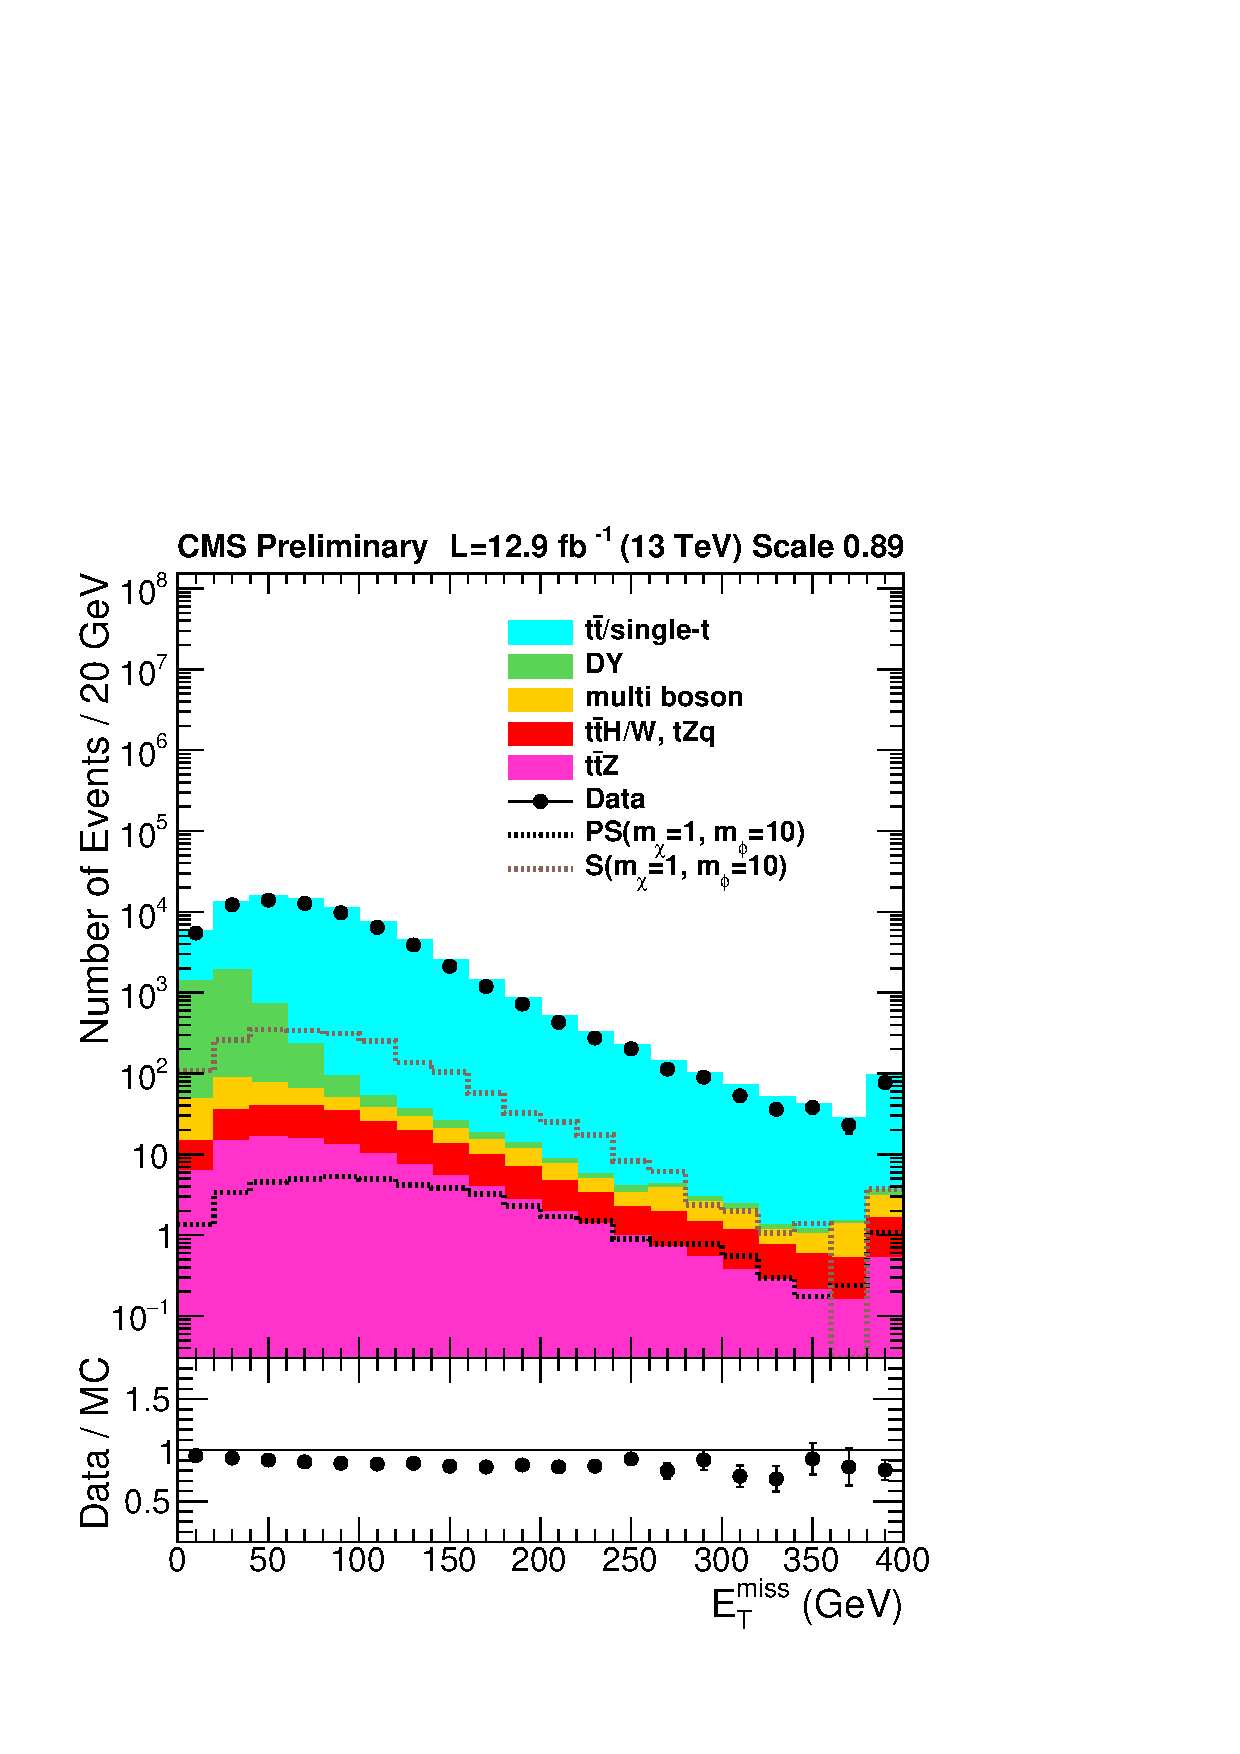
\includegraphics[width=0.45\textwidth]{figures/analysisPlots/all_log/njet2-btagM-multiIsoWP-looseLeptonVeto-mll20/met_pt.pdf}}
  \subfloat[]{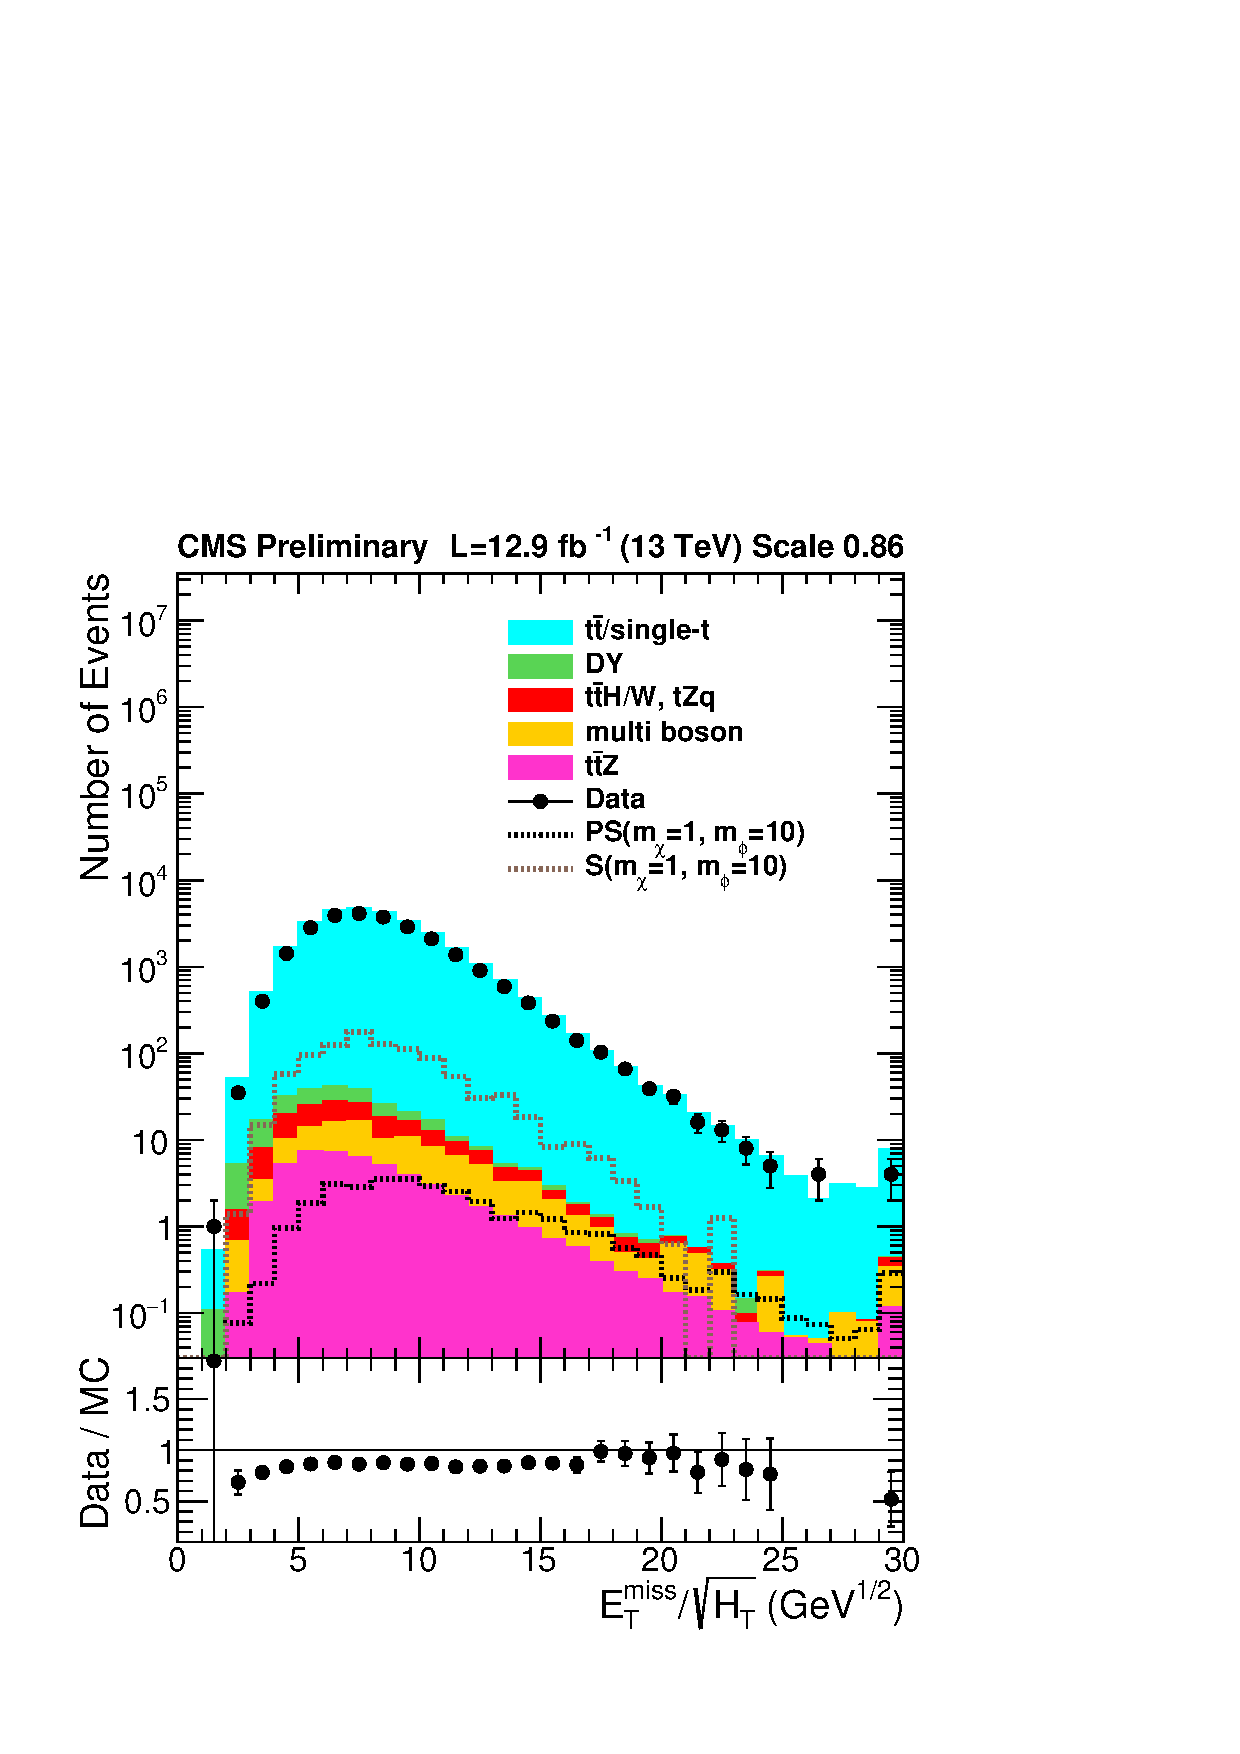
\includegraphics[width=0.45\textwidth]{figures/analysisPlots/all_log/njet2-btagM-multiIsoWP-looseLeptonVeto-mll20-met80/metSig.pdf}}
  \caption{Distributions of \met after the $m_{ll}$ selections and \metSig after the \met $>$ 80 GeV selection}\label{fig:preselMetMetSig}
  \end{figure}

  \begin{figure}
     \centering
     \subfloat[]{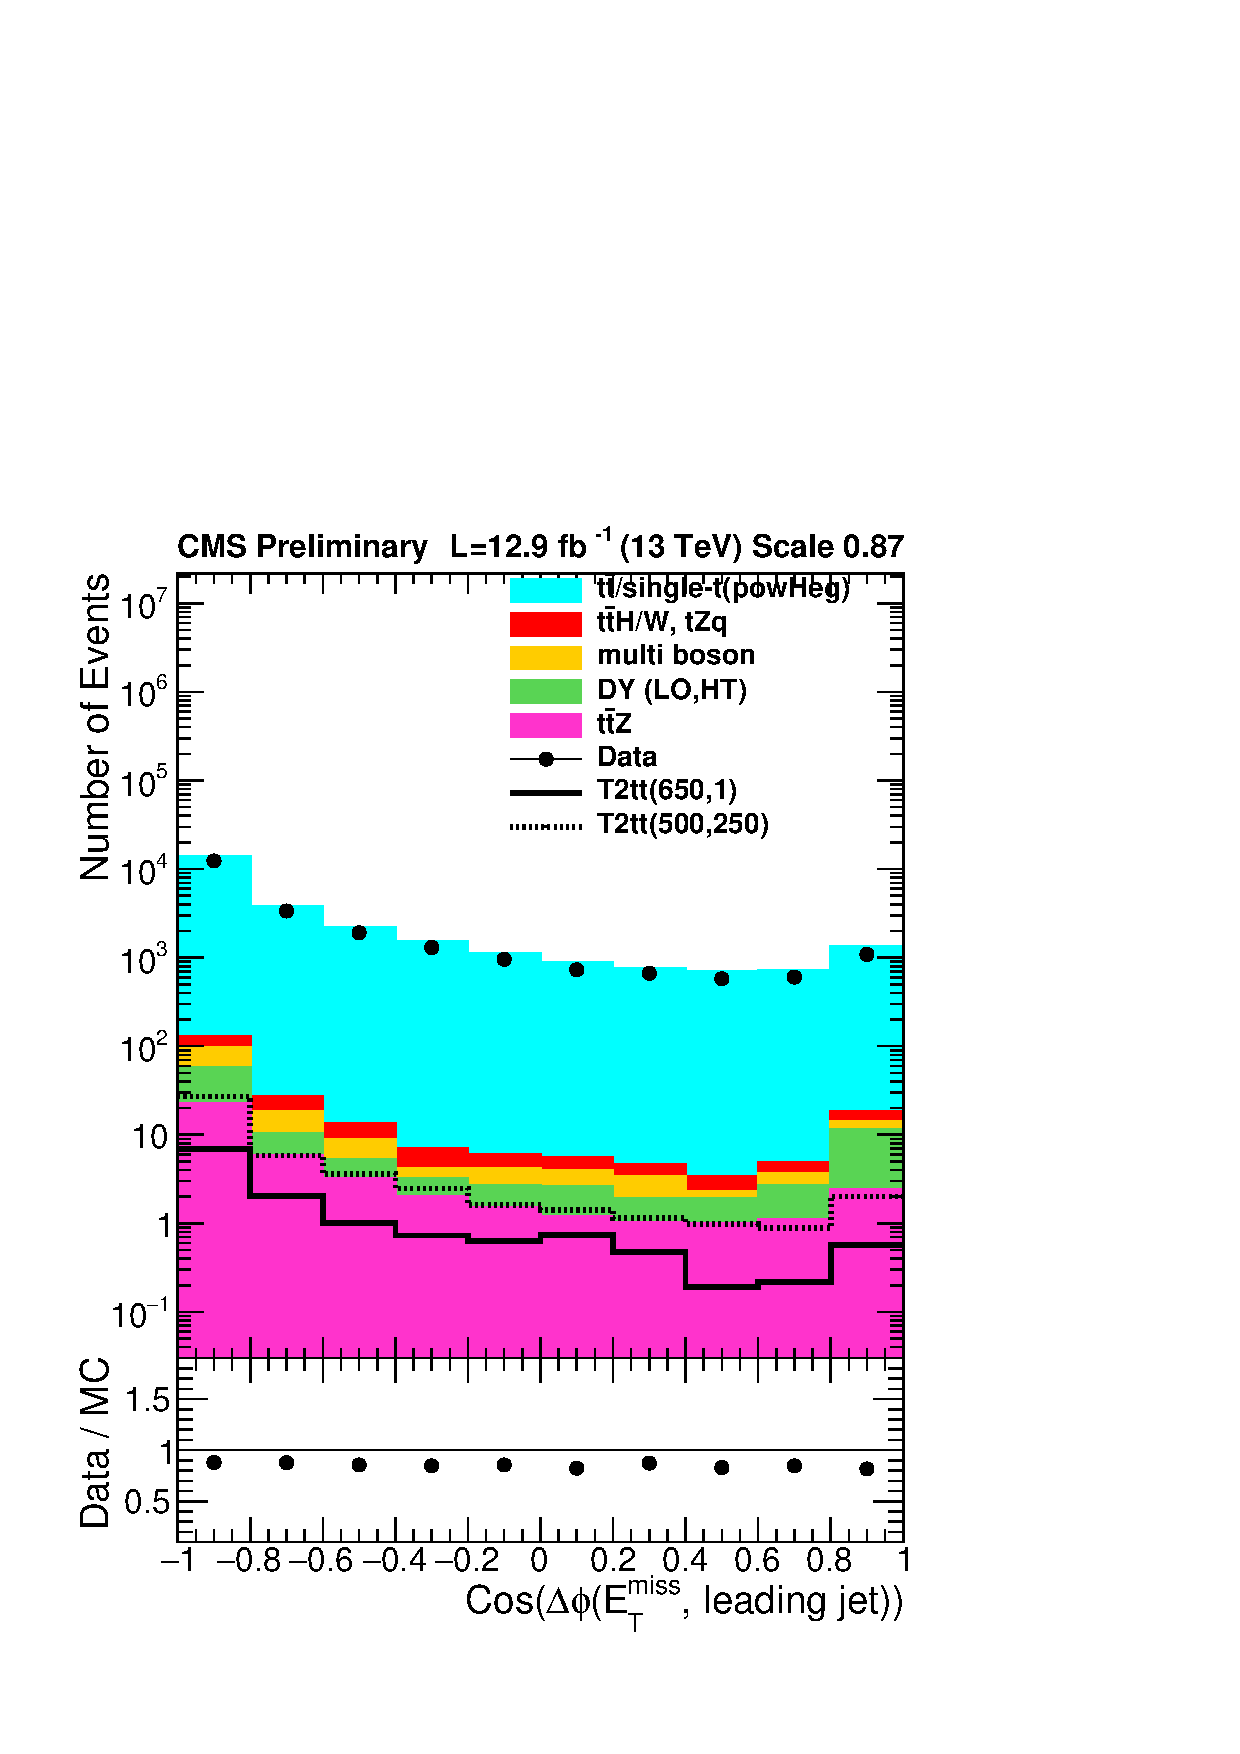
\includegraphics[width=0.45\textwidth]{figures/analysisPlots/all_log/njet2-btagM-multiIsoWP-looseLeptonVeto-mll20-met80-metSig5/cosMetJet1phi.pdf}}
     \subfloat[]{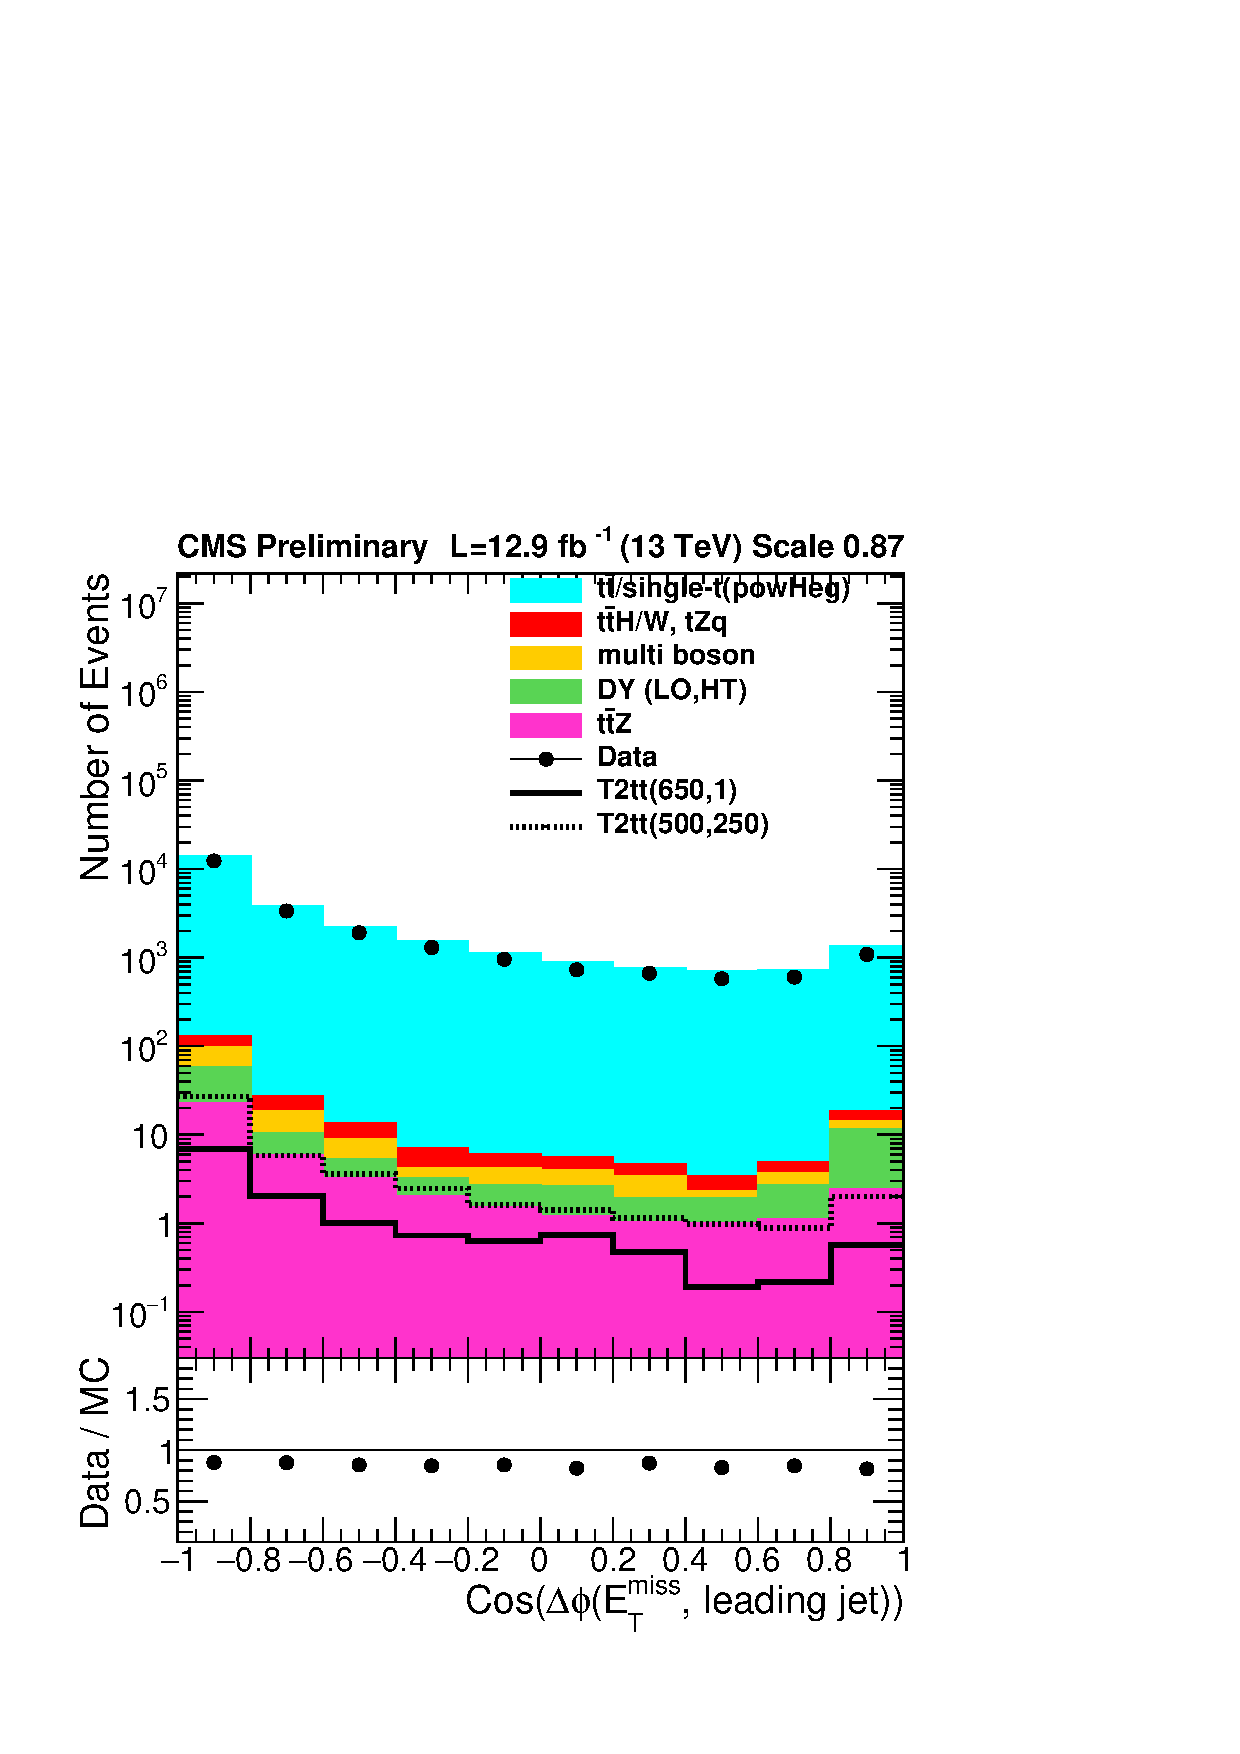
\includegraphics[width=0.45\textwidth]{figures/analysisPlots/all_log/njet2-btagM-multiIsoWP-looseLeptonVeto-mll20-met80-metSig5/cosMetJet1phi.pdf}}
     \caption{Distributions of $\cos\Delta\phi(\met, \text{j})$ for the leading and second leading jet, after the \met and \metSig selections}\label{fig:phiJetMet}
  \end{figure}

  \begin{figure}
  \centering
  \subfloat[]{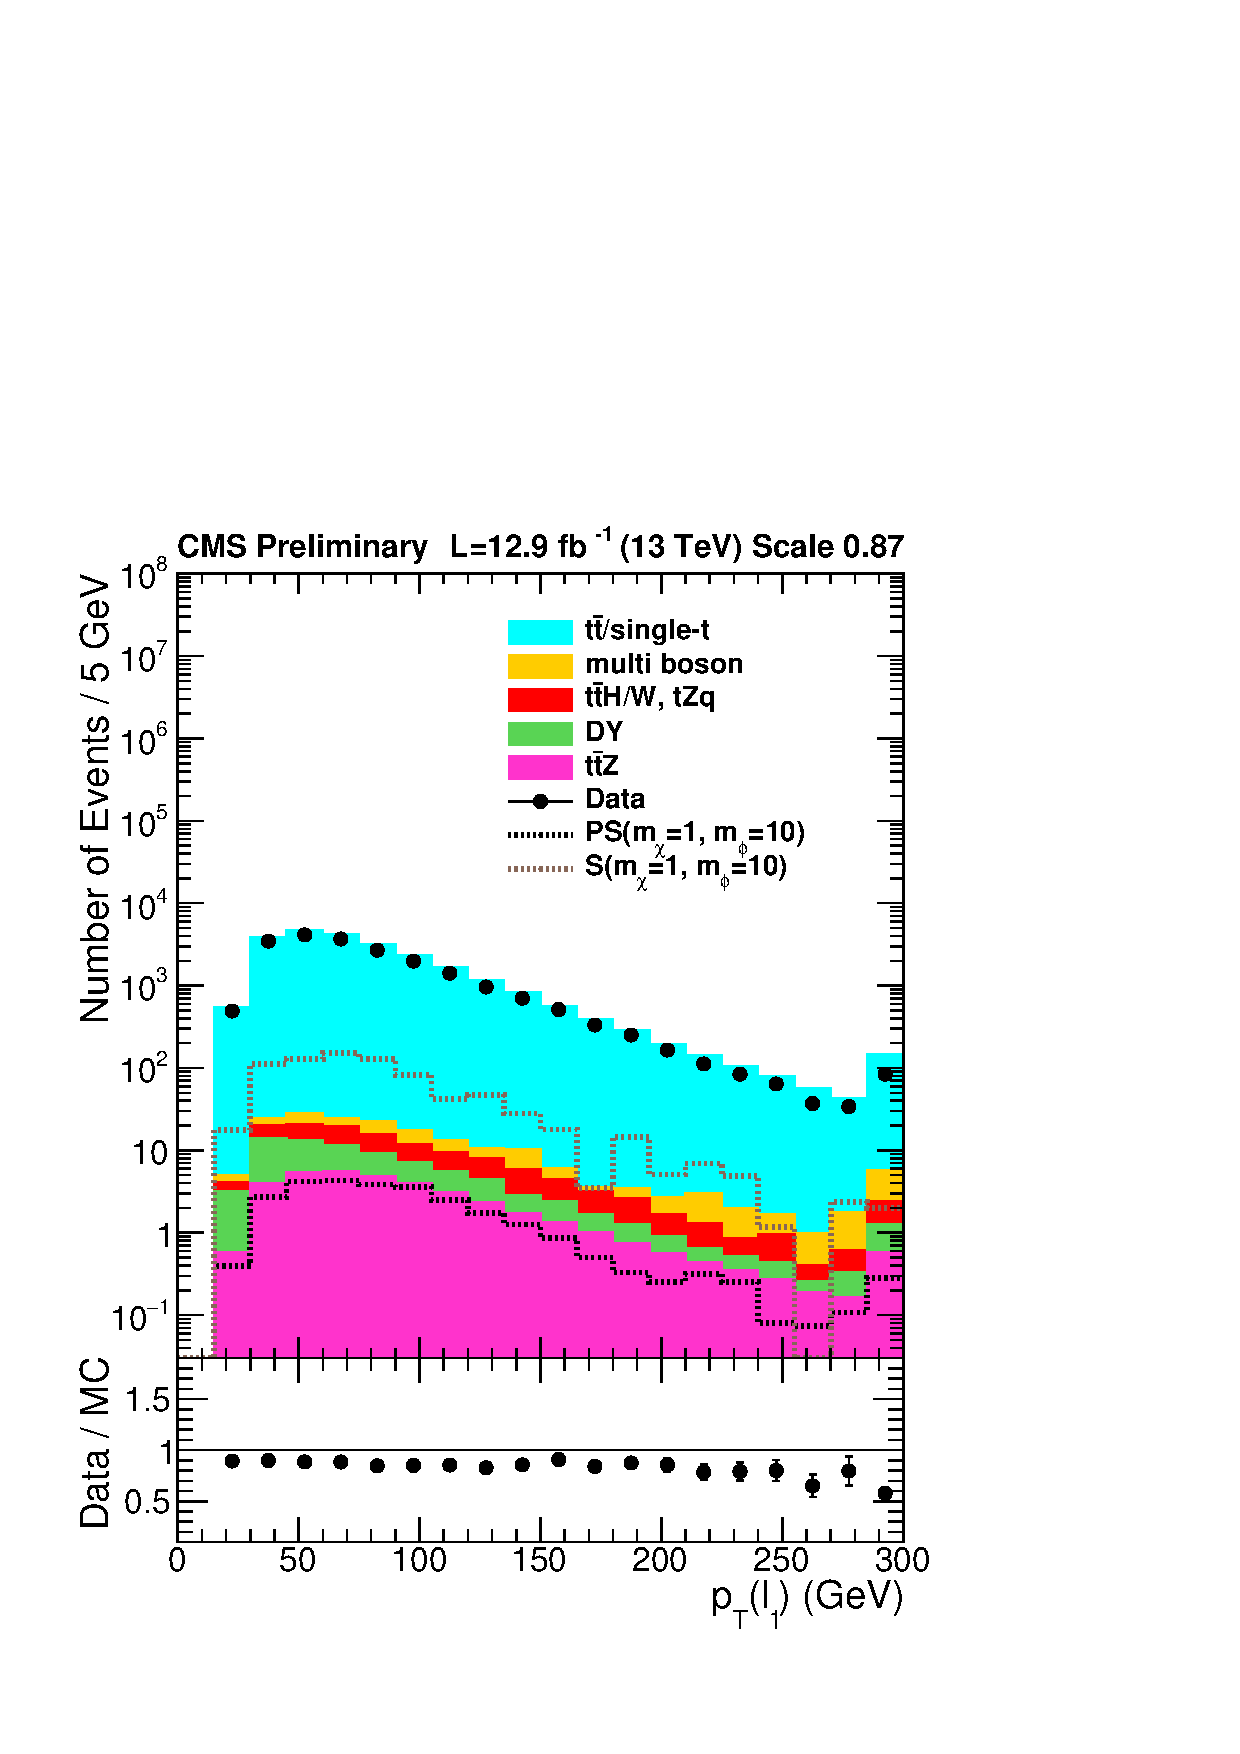
\includegraphics[width=0.45\textwidth]{figures/analysisPlots/all_log/njet2-btagM-multiIsoWP-looseLeptonVeto-mll20-met80-metSig5-dPhiJet0-dPhiJet1/l1_pt.pdf}}
  \subfloat[]{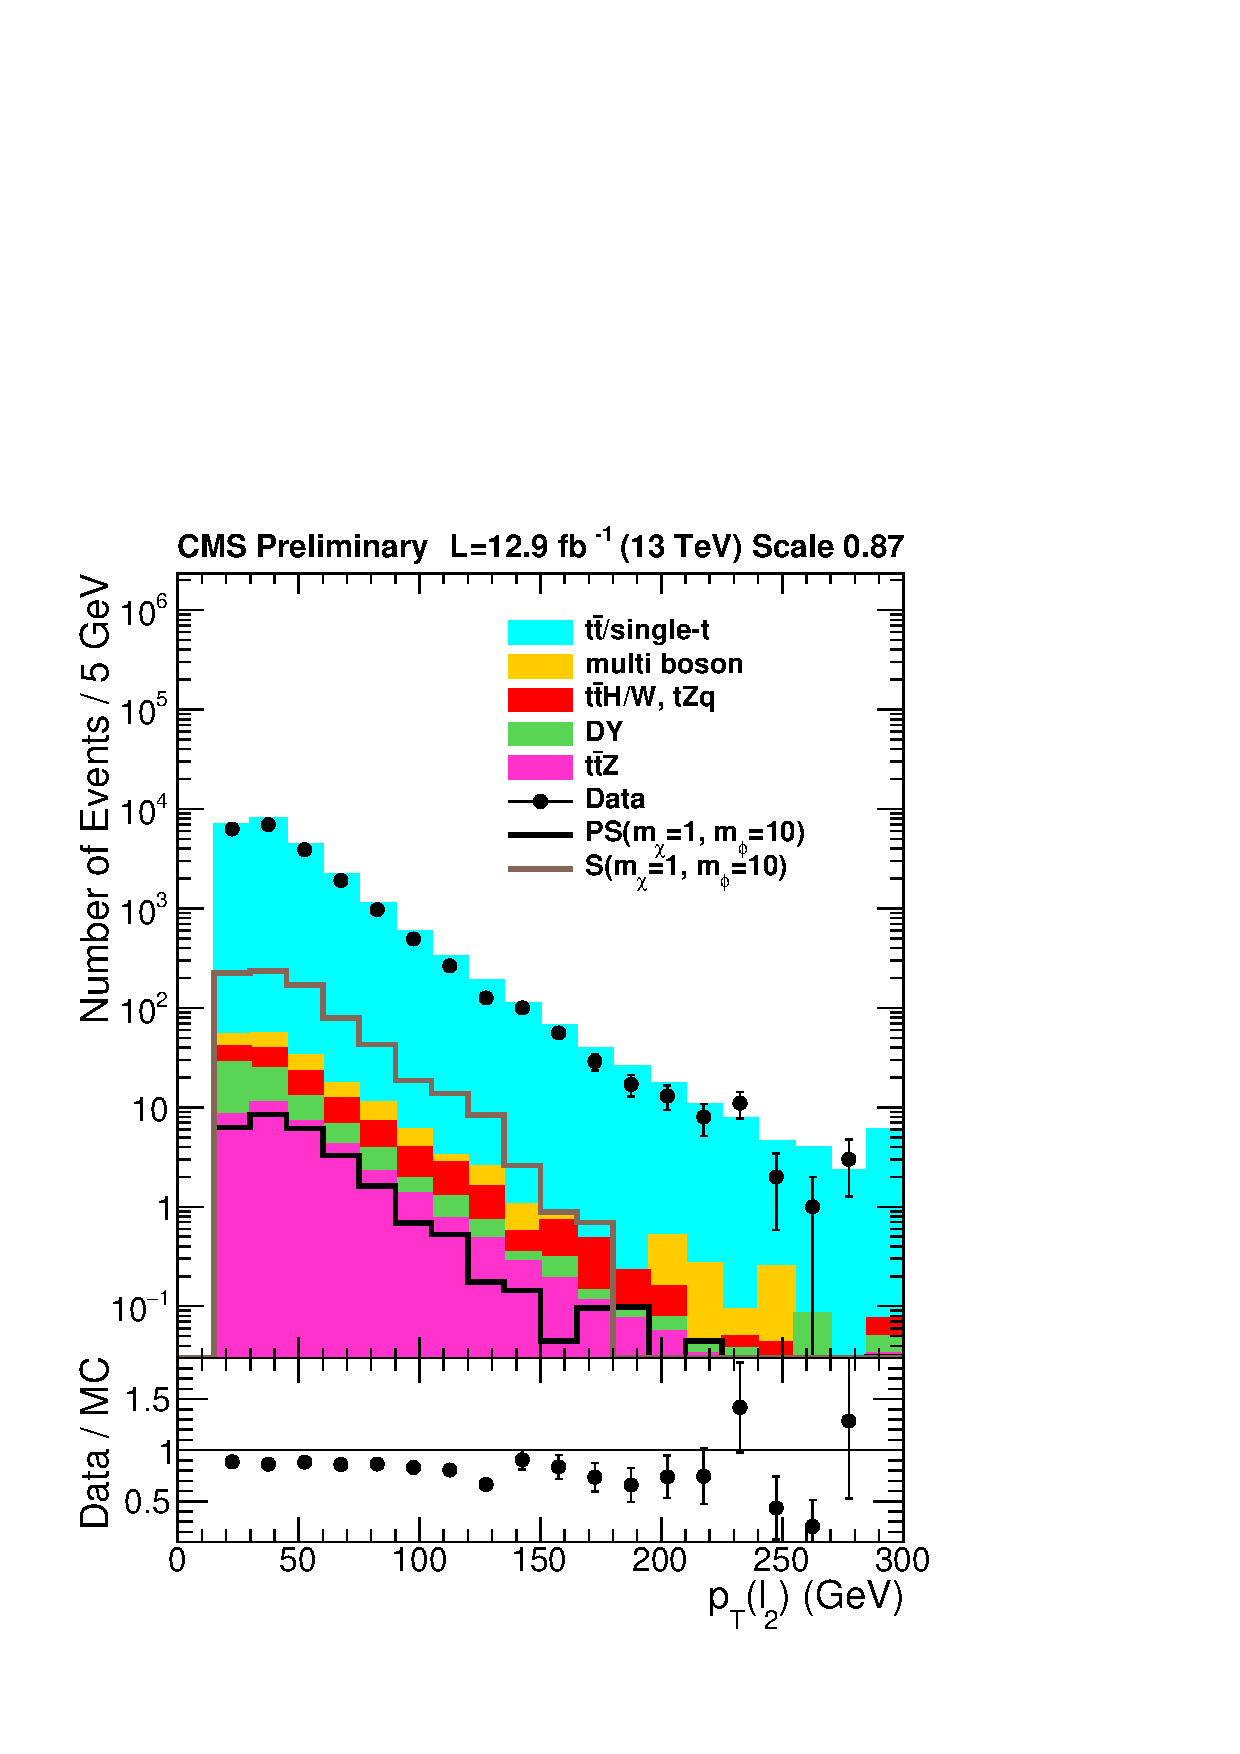
\includegraphics[width=0.45\textwidth]{figures/analysisPlots/all_log/njet2-btagM-multiIsoWP-looseLeptonVeto-mll20-met80-metSig5-dPhiJet0-dPhiJet1/l2_pt.pdf}}
  \caption{Transverse momentum distributions of the leading and second lepton after event selection}\label{fig:leptonpt}
  \end{figure}

  \begin{figure}
  \centering
  \subfloat[]{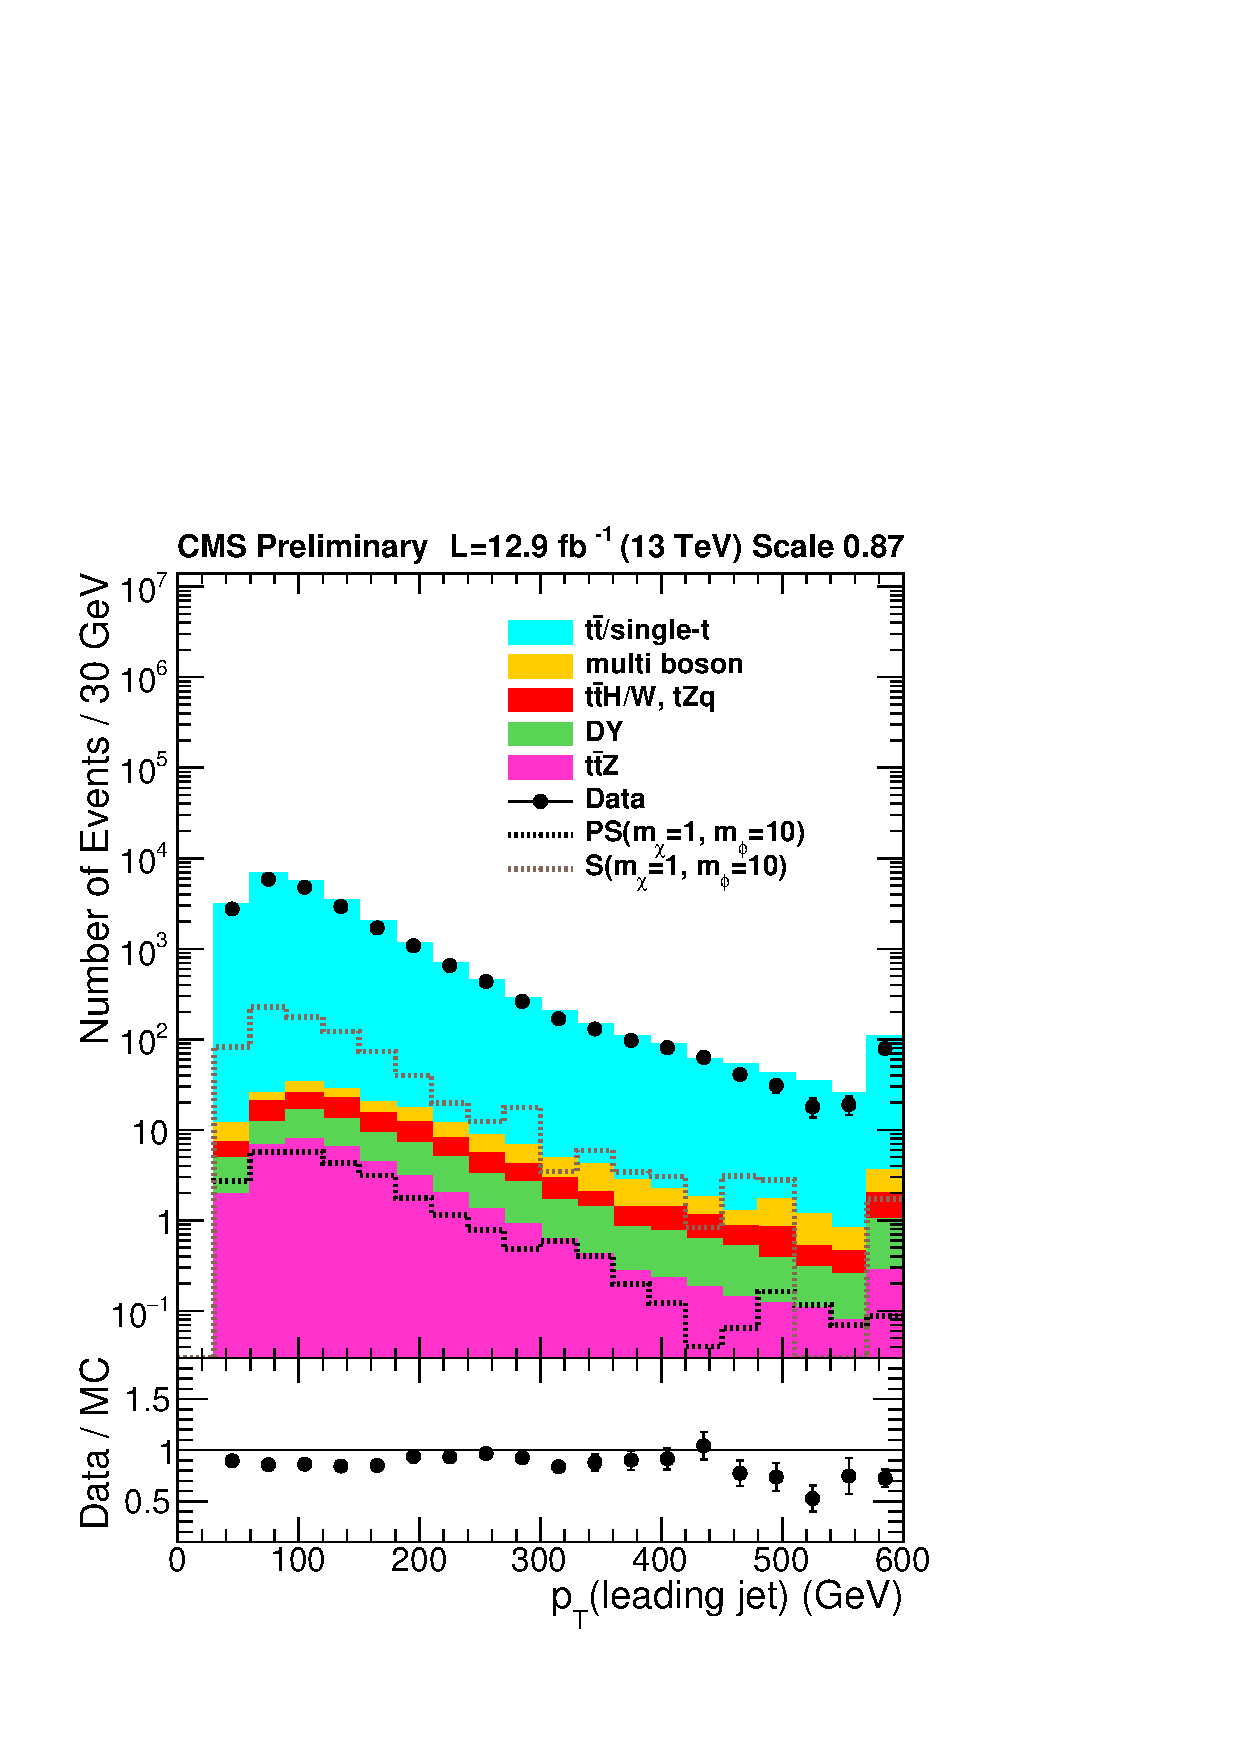
\includegraphics[width=0.45\textwidth]{figures/analysisPlots/all_log/njet2-btagM-multiIsoWP-looseLeptonVeto-mll20-met80-metSig5-dPhiJet0-dPhiJet1/jet1_pt.pdf}}
  \subfloat[]{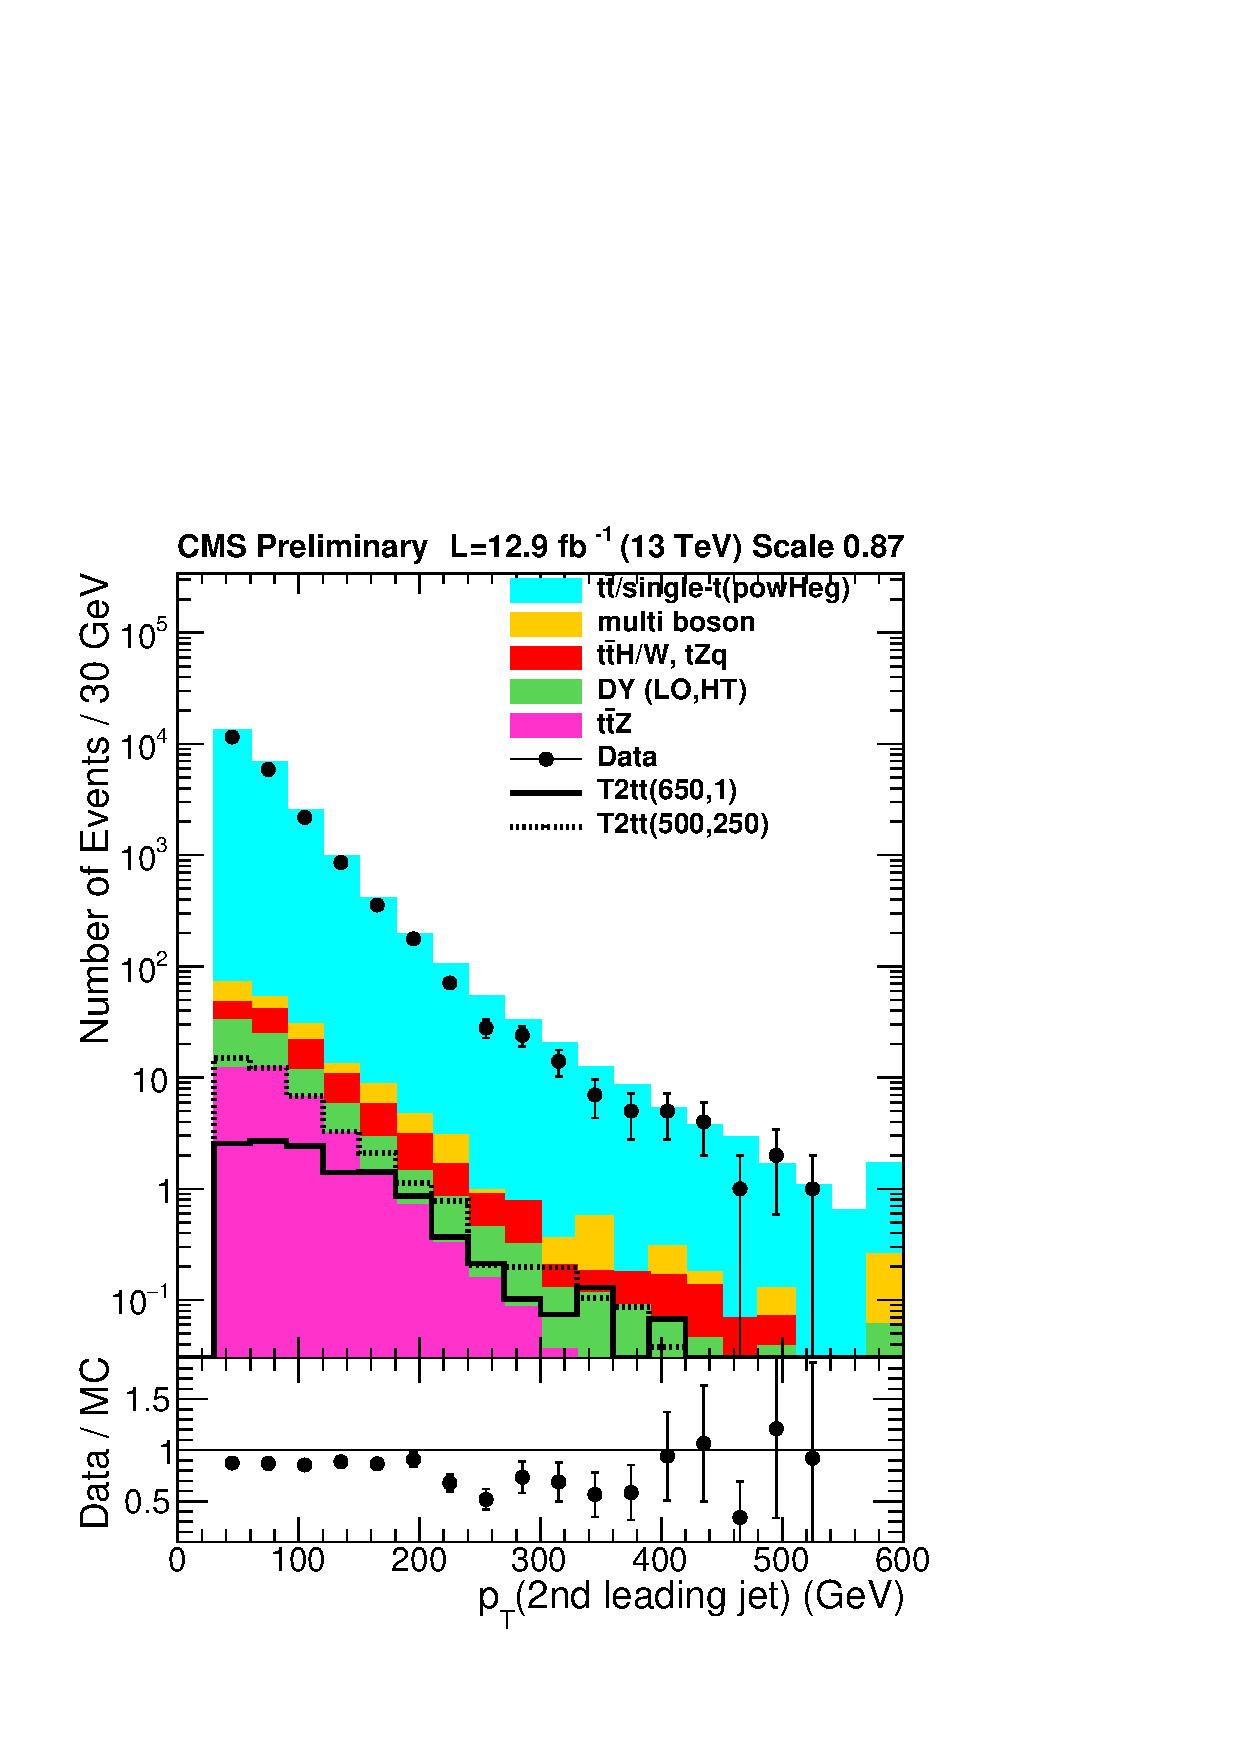
\includegraphics[width=0.45\textwidth]{figures/analysisPlots/all_log/njet2-btagM-multiIsoWP-looseLeptonVeto-mll20-met80-metSig5-dPhiJet0-dPhiJet1/jet2_pt.pdf}}
  \caption{Transverse momentum distributions of the leading and second leading jet after event selection}\label{fig:jetpt}
  \end{figure}

  \begin{table}[h]
  \setlength\tabcolsep{3pt}
  \footnotesize
  \begin{tabular}{l|ccccc|c|c|ccc}
		      &    \rotatebox[origin=c]{50}{$t\bar{t}$} &   \rotatebox[origin=c]{50}{$t\bar{t}Z$} & \rotatebox[origin=c]{50}{$t\bar{t}H/t\bar{t}W$} & \rotatebox[origin=c]{50}{multiBoson} & \rotatebox[origin=c]{50}{DY}       & \rotatebox[origin=c]{50}{total MC}      &          \rotatebox[origin=c]{50}{data} &   \rotatebox[origin=c]{50}{$S(m_\chi=1,m_\phi=10)$} & \rotatebox[origin=c]{50}{$PS(m_\chi=1,m_\phi=10)$}\\
	\hline
	2 opposite charge leptons ($e$ or $\mu$) &     135676 &        141 &        224 &      14156 &     747949 &     898144 &        854558 &      73.86 &       3379.41\\ 
	$N_\text{jets} \geq 2$                   &      92924 &        129 &        205 &       2152 &      37391 &     132802 &        128588 &      57.72 &       2568.67\\  
	$N_\text{b-jets} \geq 1$                 &      73776 &        101 &        153 &        213 &       4031 &      78274 &         69783 &      45.99 &       2019.49\\  
	$\met > 80$ GeV                          &      29179 &         49 &         77 &         66 &         84 &      29455 &         25433 &      31.75 &        963.28\\  
	$S > 5$                                  &      26972 &         42 &         61 &         59 &         59 &      27193 &         23573 &      30.50 &        889.37\\  
        $\cos\Delta\phi(\met, j_1) < 0.8$        &      25654 &         40 &         57 &         56 &         49 &      25857 &         22483 &      28.94 &        845.31\\   
	$\Delta\phi(\met, j_2) > 0.25$           &      24180 &         37 &         53 &         54 &         44 &      24367 &         21175 &      27.56 &        795.71\\
	$\mtll > 100$ GeV                        &        111 &       3.08 &       1.57 &       1.00 &       1.10 &        117 &           116 &       5.96 &         23.68\\  
	$\mtll > 140$ GeV                        &       0.78 &       1.16 &       0.45 &       0.26 &       0.29 &       2.94 &             4 &       1.89 &          4.27\\ 

    \end{tabular}
    \caption{Cutflow table showing the background, data and signal yields at the different stages of the selection}
    \label{table:yields}
  \end{table}




  \subsection{Pile-up reweighting}
  Monte Carlo events are generated according to an assumed pile-up profile and are reweighted to match the pile-up profile in data. 
  The target pile-up distribution in data is generated using the instantaneous luminosity per bunch crossing for each luminosity section
  and assuming a total $pp$ inelastic cross section of 63.2 mb~\cite{twiki:pu}. A variation of $\pm 5\%$  on this cross section is used to estimate the uncertainties due to the pile-up modeling.
  %An additional variation of 10\% was used to cross-check the PU sensitivity of the recoil modelling of DY events.

